\section{Ergebnisse}
Der Implementierung folgend konnten einige Resultate hinsichtlich der Extraktion von für die Klassifikation wichtigen Konzepten erzielt werden. Im Folgenden werden hier die unterschiedlichen Methodiken genauer betrachtet.

\subsection{Layerübergreifende Attributionen}
Für das Auffinden von Konzepten im latenten Raum des Netzwerks wurde ein Dictionary extrahiert. Dieses hält die Votings der wichtigsten Konzepte in jedem Layer über alle Beispielbilder fest.
Die Abbildung \ref{verb:latentoutput} veranschaulicht, wie sich dieses zusammensetzt; für die jeweils fünf höchsten Zählstände werden die Konzepte als \pythoninline{key-value}-Paar herausgeschnitten.

\begin{figure}[htbp]
\begin{adjustbox}{max width=0.7\linewidth}
\begin{BVerbatim}
'model_ft.features.0': {30: 40, 29: 40, 24: 40, 26: 40, 19: 40},
'model_ft.features.4': {126: 40, 121: 40, 112: 40, 106: 40, 101: 40},
'model_ft.features.8': {91: 30, 63: 27, 88: 23, 85: 20, 87: 14},
'model_ft.features.11': {240: 13, 204: 13, 63: 12, 233: 10, 93: 10},
'model_ft.features.15': {394: 8, 267: 8, 376: 8, 254: 8, 243: 7},
'model_ft.features.18': {269: 10, 254: 9, 437: 9, 225: 8, 248: 8},
'model_ft.features.22': {94: 25, 306: 24, 358: 21, 344: 12, 156: 8},
'model_ft.features.25':  {370: 40, 193: 40, 17: 38, 133: 34, 317: 22},
'model_ft.classifier.0': {3257: 40, 949: 40, 2182: 40, 1421: 39, 1191: 29},
'model_ft.classifier.3': {3641: 40, 1091: 40, 863: 40, 3137: 40, 1464: 40}
\end{BVerbatim}
\end{adjustbox}
    \caption{Dictionary-Ausgabe der layerübergreifenden wichtigsten Konzepte, gemittelt über Votings aller Samples}
    \label{verb:latentoutput}
\end{figure}
\newpage
Entsprechend können die prozentualen Relevanzen der einzelnen Konzepte in den Layern ermittelt werden; zuerst einzelne Kontributionen zur Klassifikation werden über alle Bilder gemittelt (siehe Abb. \ref{verb:latentoutput2}).
\begin{figure}[htbp]
\begin{adjustbox}{max width=\linewidth}
\begin{BVerbatim}
'model_ft.features.0': {30: 0.0, 29: 0.0, 24: 0.0, 26: 0.0, 19: 0.0}, 
'model_ft.features.4': {126: 0.0, 121: 0.0, 112: 0.0, 106: 0.0, 101: 0.0}, 
'model_ft.features.8': {91: 0.0, 63: 0.0, 88: 0.0, 85: 0.0, 87: 0.0}, 
'model_ft.features.11': {240: 0.0, 204: 0.0, 63: 0.0, 233: 0.0, 93: 0.0}, 
'model_ft.features.15': {394: 0.0001, 267: 0.0001, 376: 0.0002, 254: 0.0, 243: 0.0},
'model_ft.features.18': {269: 0.0003, 254: 0.0, 437: 0.0004, 225: 0.0001, 248: 0.0}, 
'model_ft.features.22': {94: 0.0158, 306: 0.0109, 358: 0.0021, 344: 0.0143, 156: 0.0005}, 
'model_ft.features.25': {370: 1.0575, 193: 0.8685, 17: 0.7052, 133: 0.4667, 317: 0.2513}, 
'model_ft.classifier.0': {3257: 0.3553, 949: 0.3275, 2182: 0.3204, 1421: 0.3088, 1191: 0.2223}, 
'model_ft.classifier.3': {3641: 0.3184, 1091: 0.2646, 863: 0.2565, 3137: 0.2487, 1464: 0.2396}
\end{BVerbatim}
\end{adjustbox}\caption{Dictionary-Ausgabe der Relevanzen für die wichtigsten Konzepte, gemittelt über alle Samples}
    \label{verb:latentoutput2}
\end{figure}
\begin{figure}[ht!] 
\begin{minipage}[t]{6in}
  \vspace*{.2in}
  \centering
    
\includegraphics[width=0.5\textwidth]{images/model_ft.features.8_Mitosis_152.jpg}
  \vspace*{.2in}
  
\includegraphics[width=0.5\textwidth]{images/model_ft.features.18_Mitosis_152.jpg}
    \vspace*{.2in}
  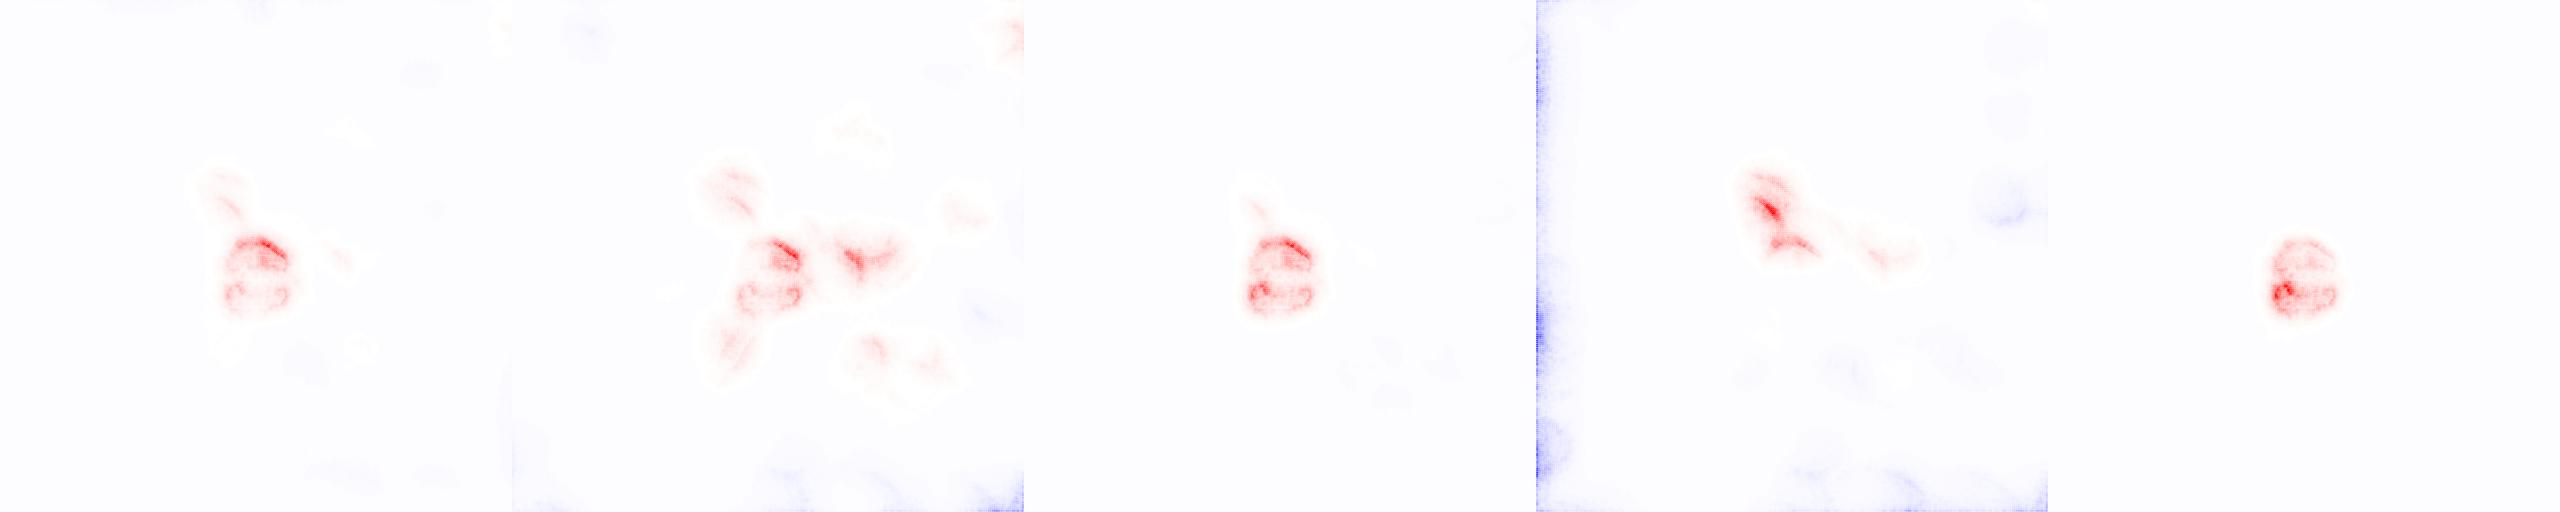
\includegraphics[width=0.5\textwidth]{images/model_ft.features.22_Mitosis_152.jpg}
  \vspace*{.2in}
    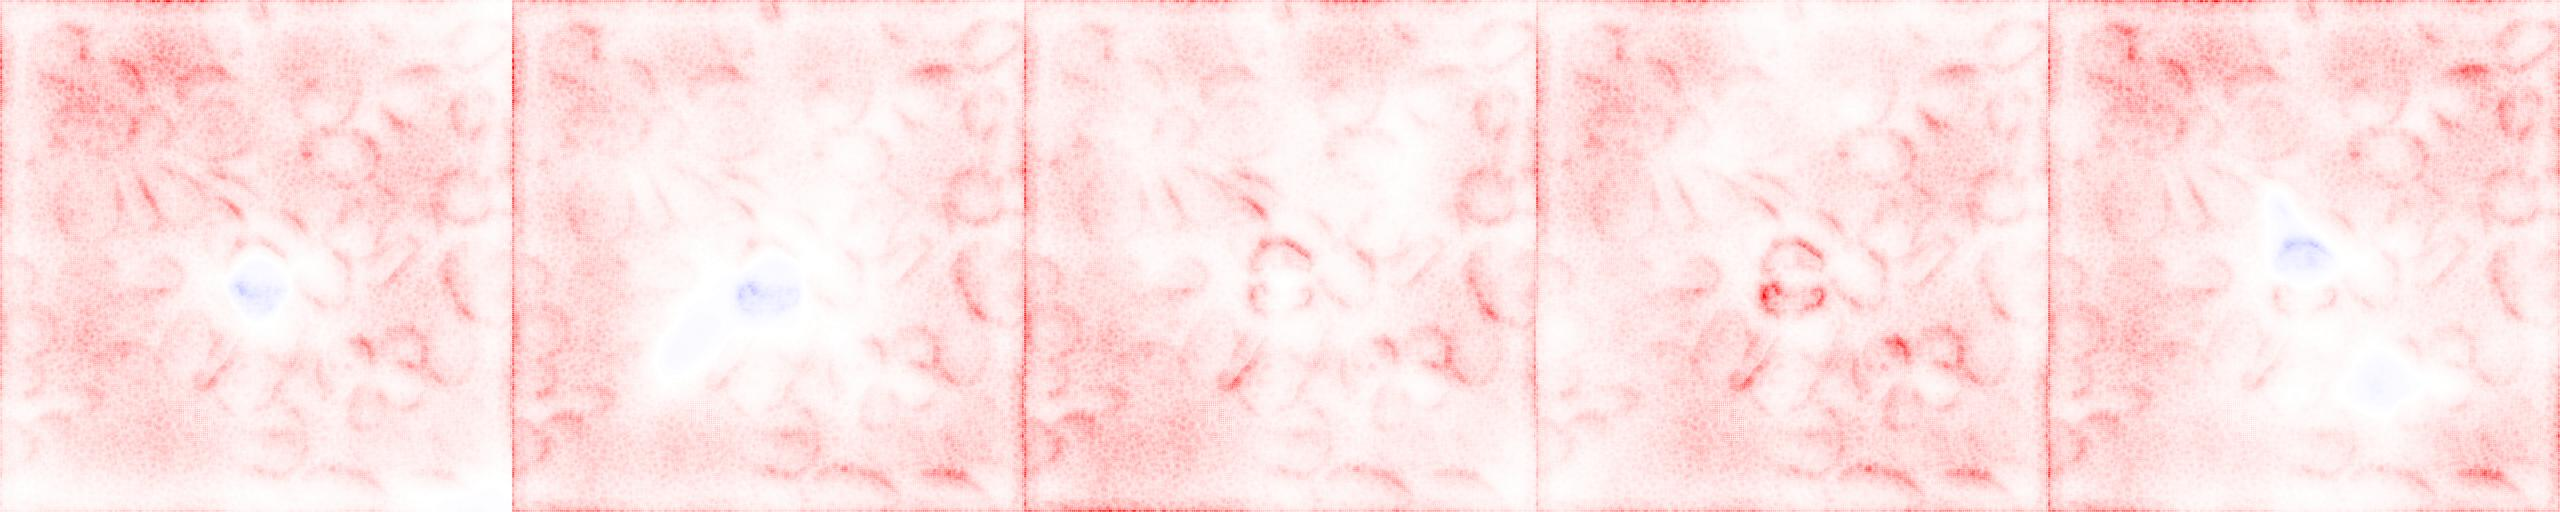
\includegraphics[width=0.5\textwidth]{images/model_ft.classifier.3_Mitosis_152.jpg}
      \vspace*{.2in}
    
\includegraphics[width=0.5\textwidth]{images/model_ft.classifier.6_Mitosis_152.jpg}
    \captionof{figure}{Konzept-Attributierungen der Layer \lstinline[breaklines=true]{features.8,features.18,features.22,classifier.3,classifier.6} für die Datei ``Mitosis\_152\_\{X=437293,Y=166519\}.jpg''}
\label{fig:latent} 
\end{minipage}
\end{figure}


Zur Visualisierung der für die Klassifikation relevanten Konzepte lassen diese sich innerhalb ihrer Layer respektive der Zielvariable {$y=1$} als Heatmap darstellen. Exemplarisch zeigt die Abbildung \ref{fig:latent}, wie hier für die Bilddatei ``Mitosis\_152\_\{X=437293,Y=166519\}.jpg''
für ein unteres, ein mittleres und ein höheres Layer des Feature-Extraktors und zwei lineare Layer des Klassifikators die Konzepte Attributionen im latenten Raum ausmachen.

\newpage
\subsection{Fragmentierung der Attributionen}
Bezüglich der Dekomposition von Konzepten, die im latenten Raum ermittelt worden sind, zeigt Abb. \ref{verb:decomoutput}, auf welchen unterliegenden Konzepte diese beruhen.

\begin{figure}[htbp]
\begin{adjustbox}{max width=0.7\linewidth}
\begin{BVerbatim}
'model_ft.features.4': {31: 40, 30: 40, 28: 40, 29: 40, 25: 40},
'model_ft.features.8': {127: 40, 126: 40, 124: 40, 125: 40, 121: 40},
'model_ft.features.11': {255: 40, 254: 40, 252: 40, 253: 40, 249: 40},
'model_ft.features.15': {154: 15, 252: 14, 95: 13, 199: 10, 175: 10},
'model_ft.features.18': {359: 13, 460: 9, 406: 8, 93: 7, 40: 7},
'model_ft.features.22': {14: 20, 366: 18, 484: 16, 364: 16, 368: 16},
'model_ft.features.25': {286: 40, 418: 40, 335: 40, 114: 40, 366: 39},
'model_ft.classifier.0': {47: 40, 331: 40, 323: 40, 133: 40, 105: 40},
'model_ft.classifier.3': {2679: 40, 779: 40, 3439: 40, 4092: 40, 2424: 25}
\end{BVerbatim}
\end{adjustbox}\caption{Dictionary-Ausgabe der für die Konzepte wichtigsten Unterkonzepte, gemittelt über alle Samples}
\label{verb:decomoutput}
\end{figure}


\newpage
\subsection{Bildregionenspezifische Attributionen}
Anhand der auf dem Bildraum maskierten Heatmap konnte auch eine lokale Analyse ein Dictionary zu wichtigen Konzepten wiedergeben (Alg. \ref{verb:localoutput}).
\begin{figure}[ht!]
\begin{adjustbox}{max width=0.7\linewidth}
\begin{BVerbatim}
'model_ft.features.0': {48: 29, 29: 29, 30: 29, 33: 28, 35: 27},
'model_ft.features.4': {52: 12, 55: 11, 25: 11, 13: 10, 20: 10},
'model_ft.features.8': {33: 14, 106: 12, 14: 11, 79: 11, 115: 9},
'model_ft.features.11': {183: 11, 154: 11, 199: 9, 229: 8, 242: 7},
'model_ft.features.15': {204: 12, 122: 10, 53: 10, 68: 10, 170: 9},
'model_ft.features.18': {76: 30, 12: 28, 256: 19, 68: 18, 366: 7},
'model_ft.features.22': {120: 39, 325: 27, 85: 23, 366: 20, 289: 19},
'model_ft.features.25': {323: 40, 193: 39, 17: 38, 26: 36, 105: 16},
'model_ft.classifier.0': {3257: 40, 949: 40, 2182: 40, 1421: 39, 1191: 29},
'model_ft.classifier.3': {3641: 40, 1091: 40, 863: 40, 3137: 40, 1464: 40}
\end{BVerbatim}
\end{adjustbox}
    \caption{Dictionary-Ausgabe der lokalen wichtigsten Konzepte, gemittelt über alle Samples}
    \label{verb:localoutput}
\end{figure}